\section{Setting up the Workspace for Java Projects}

\textbf{Objectives for this tutorial:}
\begin{itemize}
	\item create all needed library projects (runtime.java and modellib.java)
	\item create the tutorial project with the examples
	\item create the project with a traffic light simulator
	\item test the workspace setup by running one of the examples
\end{itemize}

\subsection{Create Library, Tutorial and Simulator Projects}

After installation of eclipse and the \eTrice{} plug in, your workspace should look like this:  

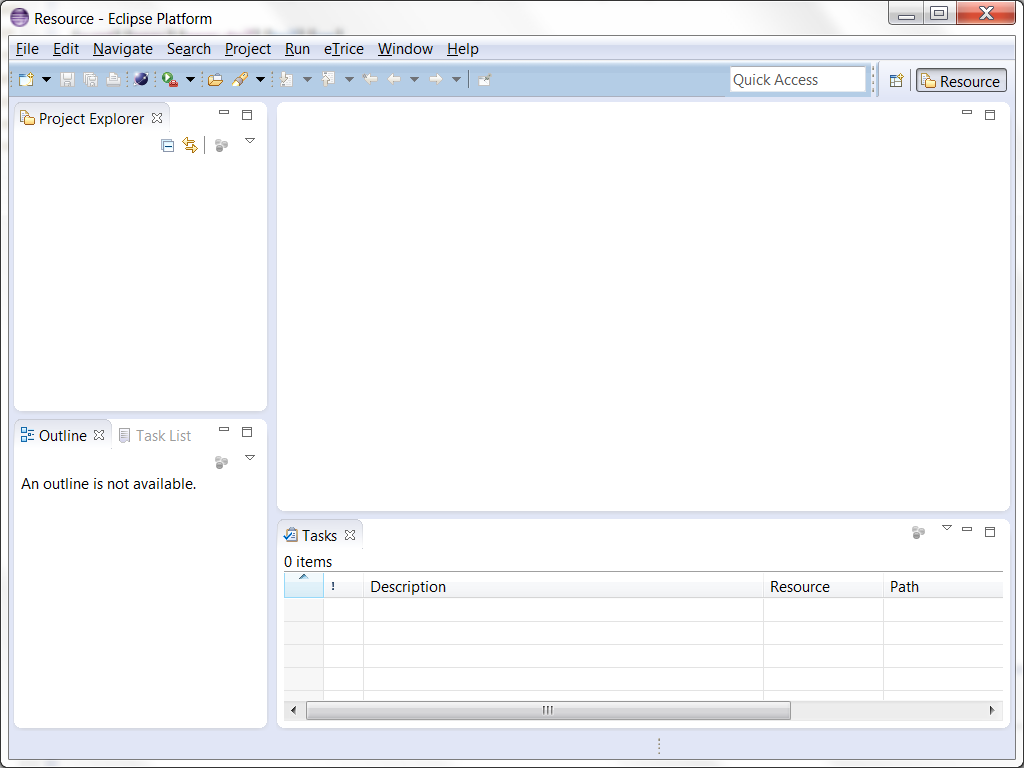
\includegraphics[width=0.8\textwidth]{images/013-SetupWorkspace01.png}
% !images/013-SetupWorkspace01.png!

Just the \eTrice{} menu item is visible of the installed \eTrice{} plugins.

\newpage
Select the menu \emph{File->New->Other}

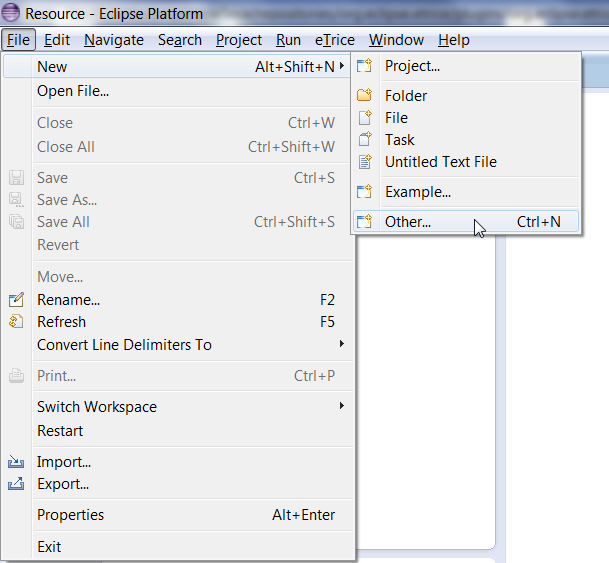
\includegraphics[width=0.6\textwidth]{images/013-SetupWorkspace02.png}
% !images/013-SetupWorkspace02.png!

Open the \emph{eTrice} tab and select \textit{eTrice Java Runtime}

Press \emph{Next} and \emph{Finish} to install the Runtime into your workspace.

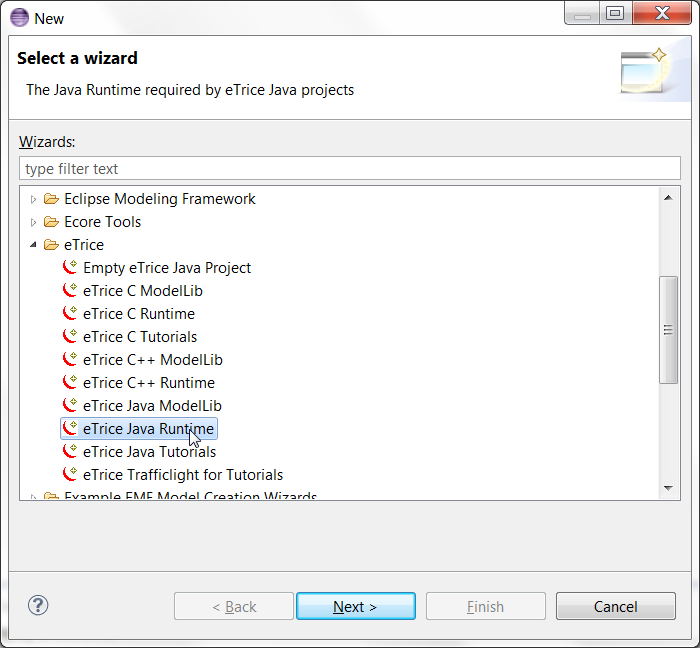
\includegraphics[width=0.6\textwidth]{images/013-SetupWorkspace03.png}
% !images/013-SetupWorkspace03.png!

\newpage
Do the same steps for \textit{eTrice Java Modellib}, \textit{eTrice Java Tutorials} and \textit{eTrice Trafficlight for Tutorials}. To avoid temporary 
error markers you should keep the proposed order of installation. The resulting workspace should look like 
this:

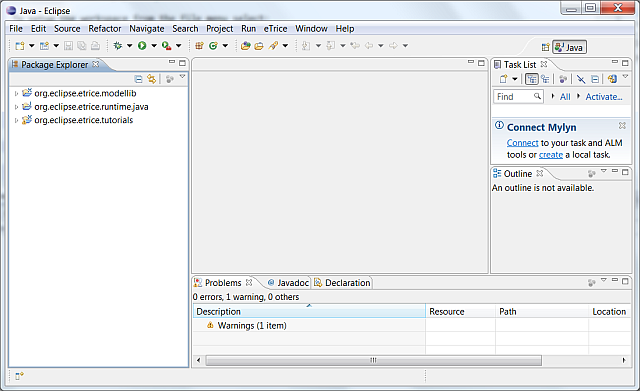
\includegraphics[width=0.5\textwidth]{images/013-SetupWorkspace04.png}
% !images/013-SetupWorkspace04.png!

\subsection{Perform Setup Test}

To check the correct setup of your workspace we run a little testproject contained in the tutorial project.

The tutorial models are available in the \textit{org.eclipse.etrice.tutorials.java} project. All tutorials are 
ready to generate and run without any changes. To test the code generator and the workspace setup simply run 
\emph{gen\_SetupTest.launch} as \emph{gen\_SetupTest}: 

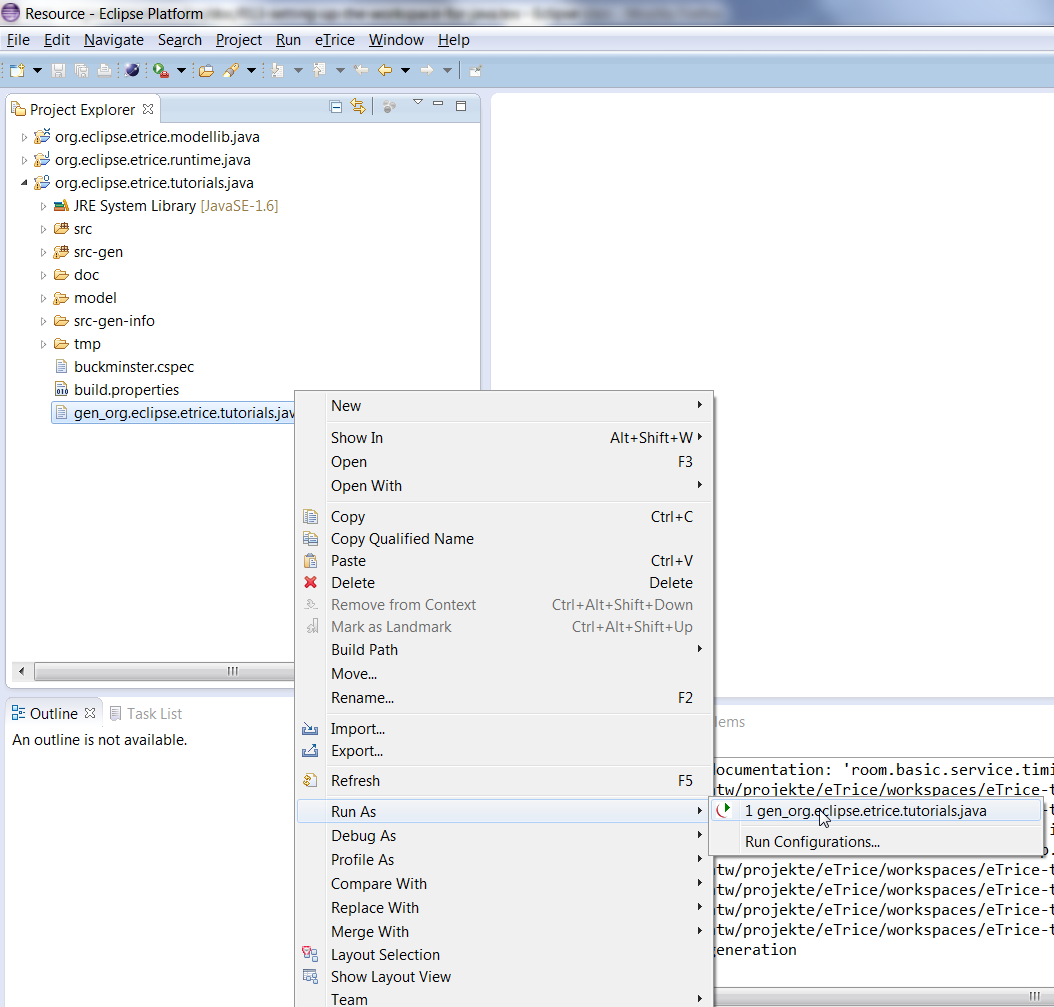
\includegraphics[width=0.6\textwidth]{images/013-SetupWorkspace05.png}
% !images/013-SetupWorkspace05.png!

\newpage
The successful generation ends with \emph{Info: -- finished code generation} in the Console.

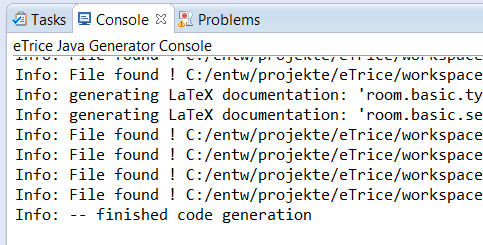
\includegraphics[width=0.5\textwidth]{images/013-SetupWorkspace051.png}
% !images/013-SetupWorkspace051.png!

For each tutorial in the folder src-gen a java package is generated including a java file called 
\emph{SubSys<...>Runner.java} . To run the generated application simply run this file as a java application.
Try this with the file \emph{src-gen/SetupTest\_Model/SubSysClass1Runner.java} :

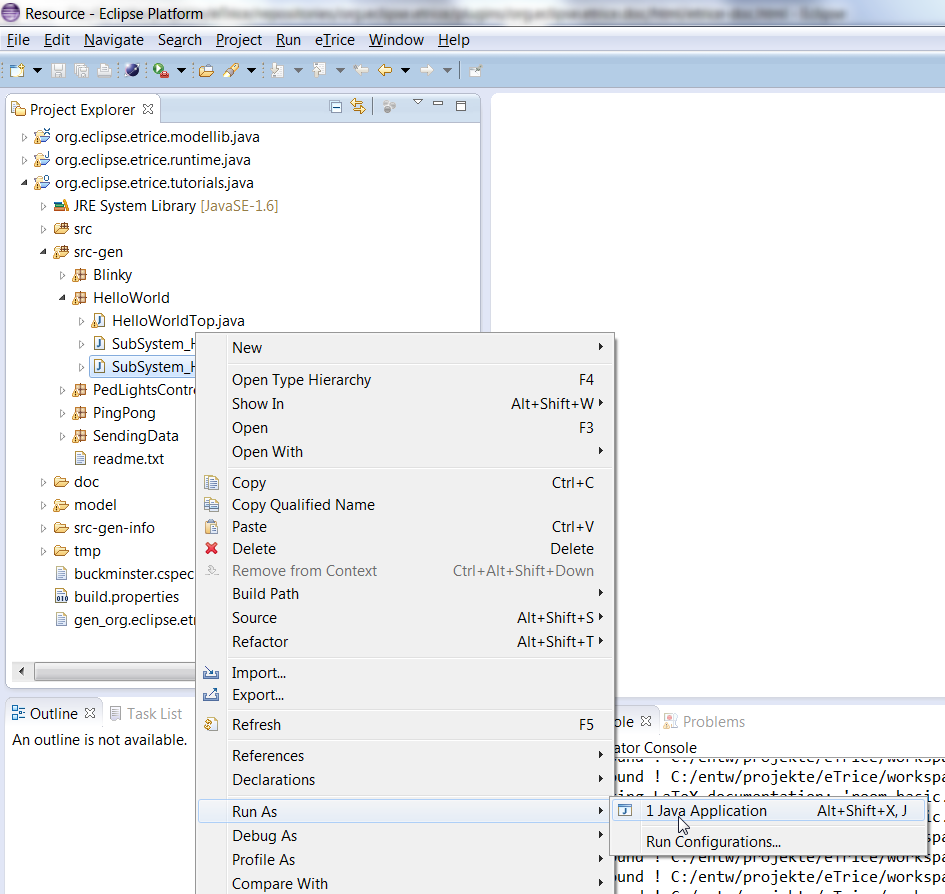
\includegraphics[width=0.6\textwidth]{images/013-SetupWorkspace06.png}
% !images/013-SetupWorkspace06.png!

To stop the application type \emph{quit} in the console window. If your Console contains the lines
\newline\emph{******************}
\newline\emph{*** Setup OK ***}
\newline\emph{******************} 
\newline your setup should be ok.
 
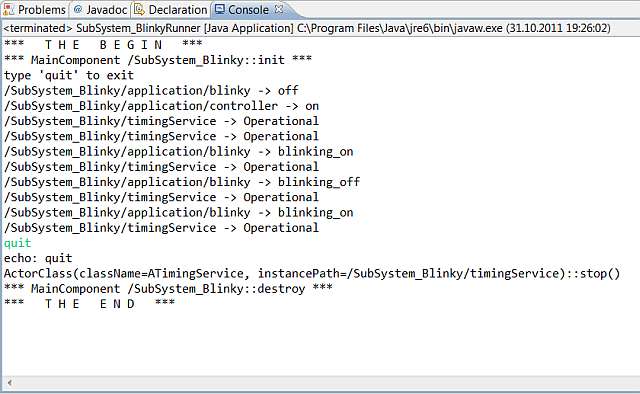
\includegraphics[width=0.6\textwidth]{images/013-SetupWorkspace07.png} 
% !images/013-SetupWorkspace07.png!

Now the workspace is set up and you can perform the tutorials or start with your work.
